\chapter{Dasar Teori}
\label{chap:teori}
Bab ini berisi dasar teori dari pembangunan Aplikasi Pencarian Rute Kendaraan Umum untuk Windows Phone. Beberapa teori yang dibahas dalam bab ini  adalah antarmuka Windows Phone, Menampilkan Peta, Penggunaan \textit{Global Positioning System} di Windows Phone, Web Service, dan Kiri API. 

% Mengenai Windows Phone
\section{Mengenai Windows Phone}
\label{sec:Mengenai Windows Phone}
\hspace{0.5cm} Windows Phone merupakan sistem operasi untuk perangkat bergerak yang dikembangkan Microsoft.\footnotemark[1] Untuk mengembangkan aplikasi Windows Phone dibutuhkan Windows Desktop 8 sebagai media pengembangan. Bahasa pemrograman yang digunakan untuk membuat perangkat lunak di Windows Phone yaitu C\# dan Visual Basic.  

\hspace{0.5cm} Pada sub bab 2.2 sampai 2.8 akan membahas pemrograman di Windows Phone. Pembahasan akan dimulai dengan apa itu Windows Phone dan fitur di Windows Phone yang akan digunakan dalam pembangunan perangkat lunak Pencarian Rute Kendaraan di Windows Phone. 
%kutipan mengenai windows phone
\footnotetext[1]{\url{en.wikipedia.org/wiki/Windows_Phone}}

% Lingkungan Kerja
\section{Lingkungan Kerja}
\label{sec:Lingkungan Kerja}
\hspace{0.5cm} Microsoft .NET framework merupakan sebuah perangkat lunak yang dibangun untuk membantu dalam pembangunan aplikasi di Windows, Windows Phone, Windows Server, and Microsoft Azure\cite{MSDN}. Ini terdiri dari runtime bahasa umum dan perpustakaan kelas NET Framework, yang meliputi kelas, interface, dan jenis nilai yang mendukung berbagai teknologi. NET Framework menyediakan lingkungan yang mudah dikelola, pengembangan disederhanakan dan penyebaran, dan integrasi dengan berbagai bahasa pemrograman, termasuk Visual Basic dan Visual C\#.

\hspace{0.5cm} Seperti yang telah disebutkan ada dua bahasa pemrograman dalam .NET Framework yang dipakai dalam pembangunan aplikasi di Windows Phone 8 yaitu Visual Basic dan Visual C\#. Untuk masalah kehandalan keduanya menawarkan kehandalan yang baik. Kelebihan dari Visual Basic adalah bahasa pemrograman berorientasi objek yang kuat dan memiliki banyak pengenbangan fitur di inheritance, polymorphism, interfaces, and overloading\cite{MSDN}.Kelebihan dari C\# yang merupakan pengembangan dari C/C++ adalah sederhana, modern, aman dan berorientasi objek\cite{MSDN}. Satu hal yang dirasakan penulis adalah kenyamanan ketika memilih bahasa .NET tersebut. Akan lebih mudah bagi developer yang menggunakan Visual Basic 6.0  untuk menggunakan Visual Basic .NET. Tetapi bagi  deveoper yang menggunakan C++ atau java sebelumnya akan lebih mudah menggunakan C\#.
%kutipan mengenai .NET
\footnotetext[2]{\url{http://msdn.microsoft.com/en-us/library/vstudio/w0x726c2\%28v=vs.110\%29}}
\footnotetext[3]{\url{http://msdn.microsoft.com/en-us/library/aa903378\%28v=vs.71\%29.aspx}}
\footnotetext[4]{\url{http://msdn.microsoft.com/en-us/library/aa287558\%28v=vs.71\%29.aspx}}

% Mengenai XAML
\section{XAML}
\label{sec:XAML}
\hspace{0.5cm} Extensible Application Markup Language (XAML) merupakan bahasa deklaratif yang dipakai untuk membuat antarmuka aplikasi. XAML merupakan bahasa yang digunakan untuk membuat antarmuka di Windows Phone 8. Pada dasarnya penggunaan XAML sama dengan HTML pada pembuatan antarmuka web. XAML dapat menginisialisasi objek dan mengatur properti untuk menunjukan hubungan antar objek.

\hspace{0.5cm} Untuk aturan penulisan sintak XAML didasarkan pada XML. Setiap XAML Windows Runtime menggunakan konvensi XAML language dan ditulis pada \textit{namespace} yang ditandai dengan prefix x sebagai elemen paling atas. Setelah itu di baris ke dua dimulai dengan xmlns diikuti titik dua, lalu nama dari \textit{namespace}, diikuti tanda sama dengan dan \textit{path} perepresentasian \textit{namespace}.
Prefix x pada XAML mengandung beberapa struktur program yang sering kita gunakan yaitu :
\begin{itemize}
	\item x:Key : sebuah nama unik untuk menunjuk referensi ke suatu resource atau berkas lain. Nilai ini dapat dipanggil kembali untuk menggunakan resource tersebut.
	\item x:Class : menunjukkan nama kelas.
	\item x:Name : menunjukkan nama sebuah obyek dan untuk membedakan antar obyek yang satu dengan obyek yang lain.
	\item x:Uid : mengidentifikasi elemen objek dalam XAML. Objek elemen merupakan objek yang dapat melakukan kontrol terhadap kelas atau elemen lain yang ditampilkan di desain anarmuka.
\end{itemize}	

% Mengenai Kontrol terhadap Ponsel
\section{Kontrol terhadap Ponsel}
\label{sec:Kontrol terhadap Ponsel}
\hspace{0.5cm} Kontrol terhadap ponsel yang dimaksudkan disini adalah pengaturan tata letak terhadap antarmuka di Windows Phone. Windows Phone 8 menyediakan banyak set kontrol yaitu tata letak, tombol, kontrol masukan untuk mendapatkan informasi sampai ke menu. 

% SUB Navigasi
\subsection{Navigasi}
\label{subsec:Navigasi}
\hspace{0.5cm} Aplikasi yang dibuat di Windows Phone didasarkan pada model halaman. Maksud dari model halaman adalah pengguna berpindah dari satu halaman ke halaman lain dengan konten yang berbeda-beda dengan frame sebagai pengontrolnya. Setiap antarmuka aplikasi dibungkus dengan frame. Frame inilah yang melakukan kontrol terhadap aplikasi dan memungkinkan berpindah dari satu halaman ke halaman lain. Sedangkan halaman merupakan pembungkus dari elemen di dalamnya saja. Untuk lebih jelas mengenai frame, halaman dan area konten dapat dilihat pada gambar di bawah ini.

\begin{figure}[h]
	\centering
		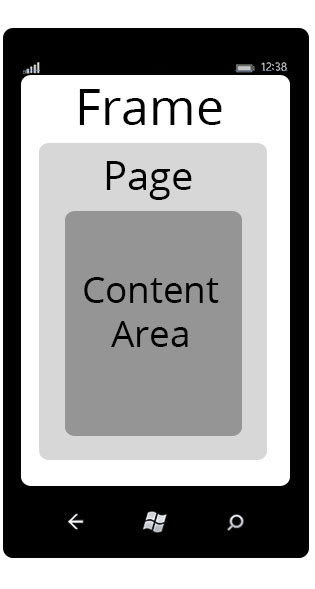
\includegraphics[scale=0.5]{Gambar/nav_hierarchy}
	\caption{Hirarki Navigasi}
	\label{fig:nav_hierarchy}
\end{figure}


% SUB Mengenai Tata Letak
\subsection{Kontrol Tata Letak}
\label{subsec:Kontrol Tata Letak}
\hspace{0.5cm} Kontrol Tata Letak merupakan penampung pada antarmuka Windows Phone untuk objek di antarmuka dan kontrol yang lain (tombol radio, textbox, dan lai-lain). Kontrol tata letak digunakan untuk meletakan objek-objek di layar. Ketika pertama membuat aplikasi Windows Phone maka tata letak dasar sebagai penampung akan langsung dibuat berikut panel judul dan panel konten. Selanjutnya untuk penambahan kontrol tata letak yang lain dapat ditambahkan di panel konten.


\hspace{0.5cm} Ada 3 macam panel yang dipakai untuk menangani Tata Letak yaitu Grid, StackPane, dan Canvas. Perlu diperhatikan bahwa setiap halaman hanya memiliki satu macam panel. Berikut 3 macam panel di Windows Phone:

\begin{itemize}
	\item StackPanel merupakan panel yang memposisikan element menjadi 1 baris dan beberapa elemen di setiap halaman diposisikan horizontal atau vertical saja.
	\item Grid merupakan panel yang mendukung tata letak yang rumit. Panel ini memposisikan elemen di baris dan kolom mana saja di setiap halaman.
	\item Canvas memposiskan elemen sebagai absolut kordinat. Jadi setiap elemen di dalam Canvas dapat diposisikan spesifik sesuai kordinat x dan y.
\end{itemize}
	
% SUB Mengenai Kontrol Masukan
\subsection{Kontrol Terhadap Teks}
\label{subsec:Kontrol Terhadap Teks}
\hspace{0.5cm} Kontrol Terhadap Teks  secara menampilkan konten String. Ada berbagai macam Kontrol Terhadap Teks di Windows Phone yaitu TextBlock, TextBox dan PasswordBox. Ketiga macam kontrol tersebut dibedakan menurut tujuannya. Berikut gambar dan keterangan masing-masing:
\begin{figure}[h]
	\centering
		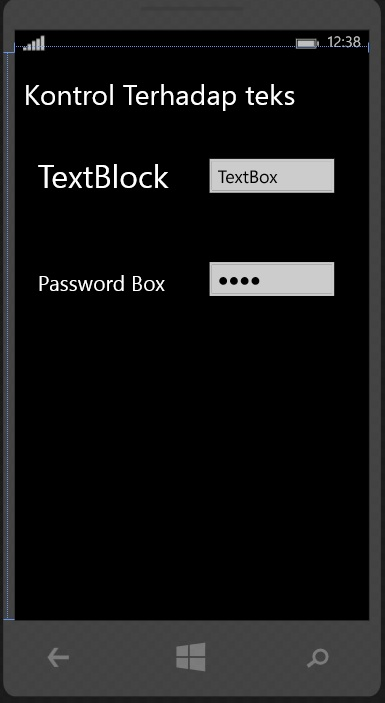
\includegraphics[scale=0.5]{Gambar/Tombol/kontrol_teks}
	\caption{TextBlock, TextBox dan PasswordBox}
	\label{fig:kontrol_teks}
\end{figure}

\begin{itemize}
	\item TextBlock merupakan tempat menaruh potongan teks yang hanya bisa dilihat.
	\item TextBox biasanya digunakan untuk teks masukan yang pendek. Tapi bisa juga dipakai untuk masukan yang banyak dan beberapa baris.
	\item PasswordBox biasanya digunakan untuk masukan yang bersifat rahasia. Karakter yang dimasukan langsung disamarkan menjadi bentuk titik.
\end{itemize}

% SUB Mengenai Kontrol Masukan
\subsection{Tombol dan Kontrol Pilihan}
\label{subsec:Tombol dan Kontrol Pilihan}
\hspace{0.5cm} Tombol memungkinkan pengguna untuk bernavigasi. Sedangkan kontrol pilihan memudahkan dalam memilih. Berikut gambar dan keterangan masing-masing:
 
\begin{figure}[h]
	\centering
		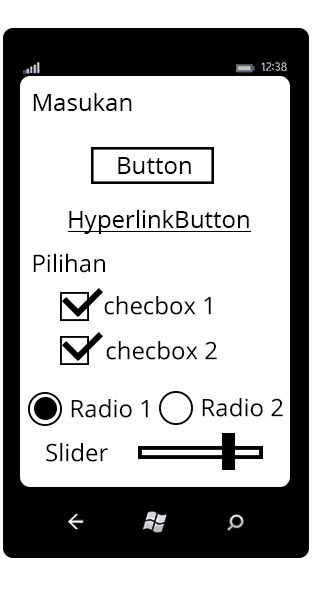
\includegraphics[scale=0.5]{Gambar/Tombol/tombol_dan_pilihan}
	\caption{TextBlock, TextBox dan PasswordBox}
	\label{fig:kontrol_tombol}
\end{figure}

\begin{itemize}
	\item Button merupakan kontrol yang dipakai pengguna untuk mengaktifkan \textit{event} klik.
	\item HyperlinkButton merupakan kontrol yang menampilkan hyperlink. Jika di tekan maka akan menunjuk ke halaman yang dituju.	
	\item CheckBox merupakan kontrol yang memungkinkan pengguna memilih beberapa item.
	\item RadioButton merupakan kontrol yang memungkinkan pengguna memilih satu pilihan dari beberapa pilihan.
	\item Slider merupakan kontrol yang memungkinkan user memilih nilai kisaran dari jalur yang sudah disediakan.
\end{itemize}

% SUB Kontrol Daftar
\subsection{Kontrol Daftar}
\label{subsec:Kontrol Daftar}
\hspace{0.5cm} Kontrol yang dipakai untuk menampilkan daftar dari beberapa item. Berikut keterangan masing-masing:

\begin{itemize}
	\item ListBox akan menampilkan daftar item. Daftar ini dapat dipilih dengan cara di klik.
	\item LongListSelector dipakai untuk mengelompokan, menampilkan, dan melakukan penggulungan terhadap daftar yang panjang.
\end{itemize}

% Mengenai Siklus Hidup Aplikasi
\section{Siklus Hidup Aplikasi}
\label{sec:Siklus Hidup Aplikasi}
\hspace{0.5cm} Siklus hidup aplikasi merupakan waktu mulai dari aplikasi dijalankan sampai aplikasi dibuang dari memori. Siklus hidup aplikasi penting diketahui agar pengguna tidak kecewa menggunakan aplikasi yang penulis buat. Seringkali pengguna tidak berhati-hati dalam menggunakan aplikasi, makadari itu penulis harus paham kapan aplikasi harus diaktifkan, ditangguhkan atau bahkan di hapus karena sudah tidak digunakan. Berikut gambar beserta keterangan siklus hidup pada Windows Phone.

\begin{figure}[h]
	\centering
		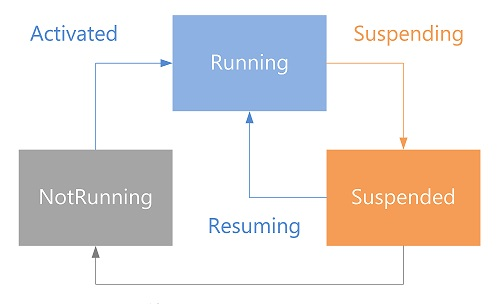
\includegraphics[scale=0.7]{Gambar/lifecycle}
	\caption{Gambar Siklus Hidup Aplikasi}
	\label{fig:Siklus Hidup Aplikasi}
\end{figure}

\begin{itemize}
	\item Running : Ketika aplikasi diluncurkan, aplikasi membutuhkan \textit{event} Activated | activated maka aplikasi akan masuk keadaan "Running". Pada saat \textit{event} Activated | activated dipanggil \textit{event} ini akan memeriksa apakah aplikasi sudah siap untuk keadaan "Running".
	\item Suspended : Aplikasi akan masuk keadaan "Suspended" ketika pengguna memilih untuk pindah aplikasi atau perangkat Windows Phone masuk ke keadaan hemat tenaga (misal: layar dimatikan sementara). Ketika pengguna berpindah aplikasi atau membuat aplikasi berjalan dibelakang layar untuk sementara waktu dan user tidak kembali ke aplikasi maka sistem operasi akan membuat aplikasi masuk ke keadaan "Suspended".
	\item Resume : Aplikasi akan masuk keadaan "Resume" ketika pengguna kembali menjalankan aplikasi atau perangkat Windows Phone keluar dari keadaan hemat tenaga (misal: layar dimatikan sementara). Saat keadaan ini semua data masih disimpan di memori jadi tidak akan ada data yang hilang.
	\item Close : Secara general pengguna tidak usah repot-repot keluar dari aplikasi karena semua sudah diurus sistem operasi. Meskipun pengguna juga dapat keluar dari aplikasi. Setelah aplikasi di keluarkan oleh pengguna dan masuk dalam keadaan "Suspended", selanjutnya aplikasi akan masuk dalam keadaan "NotRunning".
\end{itemize}

% Peta di Windows Phone
\section{Peta di Windows Phone}
\label{sec:Peta di Windows Phone}
\hspace{0.5cm} Peta yang dipakai di Windows Phone adalah Windows Phone Maps. Windows Phone menawarkan beberapa pilihan dalam tampilan peta mulai dari kartografi, pencahayaan dan pandangan. Tidak hanya tampilan pada Sub Bab ini akan dibahas mengenai mendapatkan lokasi, petunjuk arah, MapPolyline dan Pushpins.

% SUB Mengenai Penambahan Peta Ke Aplikasi
\subsection{Penambahan Peta Ke Aplikasi}
\label{subsec:Penambahan Peta Ke Aplikasi}
\hspace{0.5cm} Untuk penambahan Peta pada Windows Phone menggunakan kontrol peta. Kontrol peta merupakan bagian dari perpustakaan Windows Phone. Dengan begitu untuk dapat menggunakannya perlu direferensikan. Untuk dapat menggunakannya juga harus ditambah \textit{capability} ID\_CAP\_MAP. Selanjutnya barulah peta dapat ditampilkan.

\clearpage

\begin{figure}[h]
	\centering
		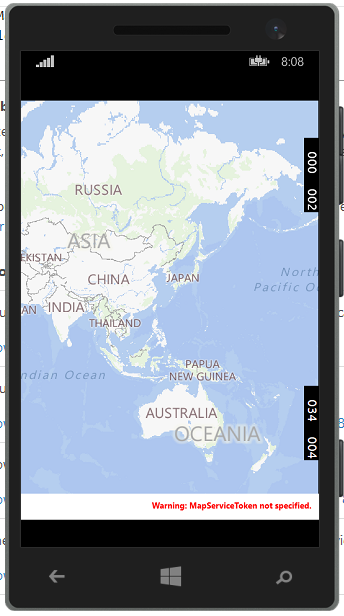
\includegraphics[scale=0.1]{Gambar/map}
	\caption{Tampilan Peta pada Windows Phone}
	\label{fig:peta}
\end{figure}

% SUB Tampilan Peta di Windows Phone
\subsection{Tampilan Peta di Windows Phone}
\label{subsec:Tampilan Peta di Windows Phone}
\hspace{0.5cm} Dalam tampilannya ada beberapa hal yang perlu diperhatikan agar pengguna merasa nyaman saat melihat peta di Windows Phone. Beberapa tampilan yang bisa ditampilkan dibuat untuk hal yang berbeda-beda. Berikut akan dibahas menentukan pusat dan tingkat zoom, kartografi, warna dan tampilan peta.

\begin{itemize}
	\item Menentukan pusat peta berarti menentukan titik tengah sebagai pandangan awal di peta. Untuk penentuan titik tengah dibutuhkan 2 nilai yaitu latitude dan longitude. Sedangkan tingkat zoom merupakan properti untuk mengatur seberapa dekat atau jauh pandangan yang akan ditampilkan di peta. Tingkat zoom memiliki nilai yang bisa diatur dari satu hingga 20. 
	\item Kartografi peta di Windows Phone merupakan cara pandang dalam melihat dan menerjemahkan peta. Ada beberapa 4 jenis kartografi, yaitu:
		
		\begin{itemize}
			\item Road: Tampilan normal 2 dimensi.
			\item Aerial: Tampilan peta yang diambil dari foto di udara.
			\item Hybrid: Tampilan Aerial yang digabung dengan jalan dan label.
			\item Terrain: Menampilkan gambar fisik bumi termasuk ketinggian dan air.
		\end{itemize}
		
		\begin{figure}[h]
			\centering
				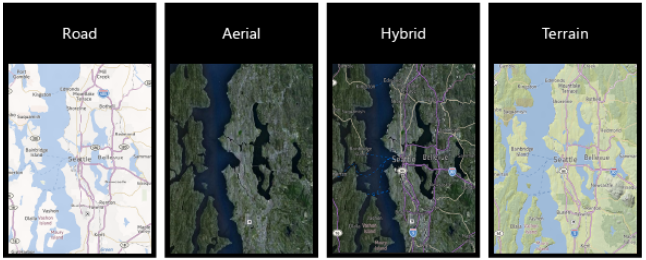
\includegraphics[scale=0.4]{Gambar/kartografi}
			\caption{Kartografi}
			\label{fig:Kartografi}
		\end{figure}
		
	\item	Mode warna yang disediakan Windows Phone ada 2 yaitu terang dan gelap. Secara bawaan mode pada peta di Windows Phone adalah terang.
	
	\item Tampilan pada Peta di Windows Phone dapat berubah karena hasil diputar, dimiringkan, ditarik, dan diturunkan. Berikut beberapa hal yang dapat diatur sebagai tampilan di peta.
	
		\begin{itemize}
			\item \textit{Heading} merupakan representasi dari derajat secara geometri. Derajat ini didefinisikan dalam 0 sampai 360 yang dipakai untuk memutar peta. Contoh, 0 atau 360 ke arah utara, 90 ke arah barat, 180 ke arah selatan, dan 270 derajat ke arah timur.
			\item \textit{Pitch} merupakan derajat kemiringan dari peta dari sudut pengguna. Contoh, \textit{Pitch} = 0 berarti melihat dari atas ke bawah sedangkan \textit{Pitch} = 45 berarti melihat dari samping ke bawah dengan sudut 45 derajat.
		\end{itemize} 
\end{itemize}

% SUB Pushpins ke Peta
\subsection{Pushpins ke Peta}
\label{subsec:Pushpins ke Peta}
\hspace{0.5cm} Pushpin merupakan elemen yang dapat ditempatkan pada peta secara spesifik dan bisa dipakai untuk interaksi pada peta. Peta tidak mendukung langsung penggunaan pushpin karena pushpin merupakan elemen MapOverlay (bagian/lapisan terpisah dari peta). Untungnya di Windows Phone memiliki Windows Phone 8 Toolkit yang memiliki set objek agar dapat menggunakan pushpin pada peta di Windows Phone. Contoh keluaran pushpin dapat dilihat pada Figure~\ref{fig:toolkit_pushpin} berikut.

\begin{figure}[!h]
	\centering
		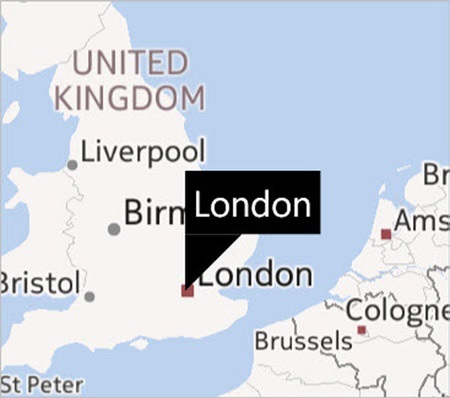
\includegraphics[scale=0.5]{Gambar/toolkit_pushpin}
	\caption{Keluaran Toolkit Pushpin pada Peta}
	\label{fig:toolkit_pushpin}
\end{figure}

% SUB Polyline pada Peta
\subsection{Polyline pada Peta}
\label{subsec:Polyline pada Peta}
\hspace{0.5cm} Dalam menentukan arah dibutuhkan 2 titik yaitu titk awal dan titik tujuan. Tentu saja arah tersebut butuh ditandai dengan garis. Polyline merupakan tentetan garis lurus yang saling terhubung satu sama lain. Dengan polyline arah pada peta dapat ditandai dengan warna maupin tebal atau tipisnya garis. 

% SUB Namespace Map
\subsection{Namespace Kontrol Map}
\label{subsec:Namespace Kontrol Map}
\hspace{0.5cm} Namespace merupakan nama yang dipakai untuk mengatur kelas-kelas. Windows Phone 8 sudah menyediakan namespace bawaan untuk mengatur peta. Namespace yang disediakan adalah Maps.Controls. Namespace ini yang berisi kelas-kelas yang paling sering digunakan untuk mengatur peta pada Windwows Phone.  Agar dapat menggunakan kelas pada namespace tersebut perlu ditambahkan namespace dan capabilities. Namespace yang harus ditambahkan pada baris awal XAML adalah Microsoft.Phone.Maps.Controls. Selanjutnya ada penambahan capabilities ID\_CAP\_MAP. Penambahan capabilities ditambahkan pada WMAppManifest.xml.

% SUB Kelas Map
\subsection{Kelas Map}
\label{subsec:Kelas Map}
\hspace{0.5cm} Merupakan kelas yang mewakili kontrol map.

Berikut properti yang dapat digunakan pada kelas ini.
\begin{table}[h]
	\centering
		\begin{tabular}{ |c||c|}
				\hline
					Nama & Deskripsi \\ \hline
					CartographicMode & Mengatur dan mendapatkan tipe dari peta. \\ \hline
					Center & Mengatur dan mendapatkan lokasi tengah pada peta. \\ \hline
					ColorMode & Mengatur dan mendapatkan mode warna peta \\ \hline
					Heading & Mengatur dan mendapatkan arah pandang peta. \\ \hline
					Height & Mengatur dan mendapatkan tinggi. \\ \hline
					LandmarksEnabled & Mengindikasikan apakah bangunan 3D ditampilkan. \\ \hline
					Name & Mengatur dan mendapatkan nama identifikasi objek. \\ \hline
					PedestrianFeaturesEnabled & Mengindikasikan fitur pejalan kaki ditampilkan. \\ \hline
					Pitch & Mengatur dan mendapatkan derajat kemiringan peta. \\ \hline
					Tag & Mengatur dan mendapatkan nilai objek. \\ \hline
					TileSources & Mendapatkan koleksi lapisan lantai. \\ \hline
					Width & Mengatur dan mendapatkan lebar. \\ \hline
					ZoomLevel & Mengatur dan mendapatkan tingkat zoom pada peta. \\ \hline
				\hline
		\end{tabular}
	\caption{Properti Kelas Map}
	\label{tab:PropertiKelasMap}
\end{table}

Berikut metode yang dapat digunakan pada kelas ini.
\begin{itemize}
	\item SetView(LocationRectangle) \\
	Metode untuk mengatur pandangan di atas peta secara spesifik sesuai region geografis. Metode ini tidak mengambalikan nilai.
	\item SetView(GeoCoordinate, Double) \\
	Metode untuk mengatur pandangan di atas peta secara spesifik sesuai titik tengah dan tingkat zoom. Metode ini tidak mengambalikan nilai.
	\item SetView(LocationRectangle, MapAnimationKind)\\
	Metode untuk mengatur pandangan di atas peta secara spesifik sesuai region geografis dan animasi. Metode ini tidak mengambalikan nilai.
	\item 	SetView(LocationRectangle, Thickness) \\
	Metode untuk mengatur pandangan di atas peta secara spesifik sesuai region geografis dengan batas tertentu. Metode ini tidak mengambalikan nilai.
	\item 	SetView(GeoCoordinate, Double, MapAnimationKind) \\
	Metode untuk mengatur pandangan di atas peta secara spesifik sesuai titik tengah, tingkat zoom, dan animasi. Metode ini tidak mengambalikan nilai.
	\item 		SetView(GeoCoordinate, Double, Double) \\
	Metode untuk mengatur pandangan di atas peta secara spesifik sesuai titik tengah, tingkat zoom, dan heading. Metode ini tidak mengambalikan nilai.
	\item 		SetView(LocationRectangle, Thickness, MapAnimationKind) \\
	Metode untuk mengatur pandangan di atas peta secara spesifik sesuai region geografis dengan batas tertentu, dan animasi. Metode ini tidak mengambalikan nilai.
	\item 		SetView(GeoCoordinate, Double, Double, MapAnimationKind) \\
	Metode untuk mengatur pandangan di atas peta secara spesifik sesuai titik tengah, tingkat zoom, heading, dan animasi. Metode ini tidak mengambalikan nilai.	
	\item SetView(GeoCoordinate, Double, Double, Double) \\
	Metode untuk mengatur pandangan di atas peta secara spesifik sesuai titik tengah, tingkat zoom, heading, pitch. Metode ini tidak mengambalikan nilai.
	\item 	SetView(GeoCoordinate, Double, Double, Double, MapAnimationKind) \\
	Metode untuk mengatur pandangan di atas peta secara spesifik sesuai titik tengah, tingkat zoom, heading, pitch, dan animasi. Metode ini tidak mengambalikan nilai.
	\item UpdateLayout \\
	Metode yang memastikan semua posisi objek turunan mengikuti tata letak. 
\end{itemize}

% SUB Kelas Polyline
\subsection{Kelas Polyline}
\label{subsec:Kelas Polyline}
\hspace{0.5cm} Merupakan kelas yang dipakai untuk menggambarkan garis lurus yang saling terhubung. Kelas ini tergabung ke dalam namespace  Microsoft.Phone.Maps.Controls. 

Berikut properti yang dapat digunakan pada kelas ini.
\begin{table}[h]
	\centering
		\begin{tabular}{ |c||c|}
				\hline
					Nama & Deskripsi \\ \hline
					Dispacher & Mendapatkan objek yang terkait. \\ \hline
					Path & Mengatur dan mendapatkan kumpulan GeoCoordinates yang membuat polyline. \\ \hline
					StrokeColor & Mengatur dan mendapatkan warna garis. \\ \hline
					StrokeDashed & Mengatur dan mendapatkan nilai untuk mengetahui jika polyline dihancurkan. \\ \hline
					StrokeThickness & Mengatur dan mendapatkan lebar garis untuk menggambar polyline. \\ \hline
				\hline
		\end{tabular}
	\caption{Properti Kelas Polyline}
	\label{tab:PropertiKelasPolyline}
\end{table}

Berikut metode yang dapat digunakan pada kelas ini.
\begin{itemize}
	\item CheckAccess\\
	Metode yang menentukan bisa atau tidaknya pemanggilan thread untuk mengakses objek ini.
	\item ClearValue\\
	Metode yang akan membersihkan nilai lokal
	\item Finalize \\
	Metode yang dipakai untuk melakukan pembersihan pada sumber daya yang tidak terpakai sebelum objek dihancurkan.
\end{itemize}

% SUB Kelas Pushpin
\subsection{Kelas Pushpin}
\label{subsec:Kelas Pushpin}
\hspace{0.5cm} Merupakan kelas yang dipakai untuk menggambarkan ?????

% Lokasi
\section{Lokasi}
\label{sec:Lokasi}
\hspace{0.5cm} Aplikasi di Windows Phone 8 dapat memanfaatkan lokasi dimana perangkat berada. Aplikasi dapat melacak lokasi sesaat  pengguna atau pelacakan selama periode tertentu. Data lokasi perangkat berasal dari berbagai sumber termasuk \textit{Global Positioning System} atau GPS, Wi-Fi, dan seluler. Ada 2 set API berbeda yang dapat dimanfaatkan di Windows Phone yaitu \textit{Runtime Location} API dan .NET \textit{Location} API. Windows Phone \textit{Runtime Location} memiliki keunggulan fitur yang banyak sedangkan .NET \textit{Location} direkomendasikan jika aplikasi ditargetkan pada Windows Phone 7.1 dan Windows Phone 8.

\hspace{0.5cm} Hal yang perlu diperhatikan dalam menentukan layanan lokasi adalah penangkap GPS, Wi-Fi, dan radio seluler. Perangkat tersebut berfungsi sebagai penyedia data lokasi dengan berbagai tingkat akurasi dan konsumsi daya. Perangkat diatas juga berkomunikasi langsung untuk memutuskan sumber mana yang digunakan untuk menentukan lokasi perangkat berdasarkan ketersediaan data lokasi dan prasyarat yang ditentukan aplikasi. Lapisan diatas penyedia data lokasi tersebut adalah pengelola antarmuka. Aplikasi akan mengunakan antarmuka tersebut untuk memulai dan menghentikan layanan lokasi, mengatur tingkat akurasi, dan menerima data lokasi.

% SUB Mendapatkan Posisi Pengguna
\subsection{Mendapatkan Posisi Pengguna}
\label{subsec:Mendapatkan Posisi Pengguna}
\hspace{0.5cm} Di Windows Phone 8 telah ada GeoCoordinate yang dapat digunakan untuk mengetahui posisi pengguna. Geolocator dari Windows.Devices.Geolocation akan mengembalikan posisi saat ini. Untuk menggunakan Geolocator, perlu menghidupkan ID\_CAP\_LOCATION di \textbackslash properties\textbackslash WMAppManifest.xml. Dalam mendapatkan posisi juga perlu diperhatikan status dari GPS karena GPS membutuhkan waktu dari mengaktifkan GPS hingga mendapatkan lokasi pengguna secara akurat. Untuk lebih jelas mengenai status dalat dilihat pada nilai status dibawah ini.

Berikut nilai yang mungkin dari Status Posisi:
\begin{itemize}
	\item \textit{Ready} : Jika lokasi tersedia.
	\item \textit{Initializing} : Status jika penangkap GPS belum memiliki cukup satelit untuk mendapatkan posisi yang akurat. 
	\item \textit{NoData} : Data lokasi belum tersedia. Status ini muncul jika aplikasi sedang mamanggil GetGeopositionAsync atau register.
	\item \textit{Disable} : Status mengindikasikan tidak diperbolehkannya pengaksesan lokasi.
	\item \textit{NotInitialized} : Data lokasi belum tersedia. Status ini muncul jika aplikasi belum mamanggil GetGeopositionAsync atau register.
	\item \textit{NotAvailable} : Jika Windows sensor dan lokasi tidak tersedia.
\end{itemize}

% SUB Namespace Geolocator
\subsection{Namespace Geolocator}
\label{subsec:Namespace Geolocator}
\hspace{0.5cm} Namespace merupakan nama yang dipakai untuk mengatur kelas-kelas. Windows Phone 8 sudah menyediakan namespace bawaan untuk mengakses lokasi. Namespace yang disediakan adalah namespace Geolocator. Namespace ini akan mengakses lokasi geografis dari perangkat dan mendukung pelacakan lokasi dari waktu ke waktu. Agar dapat menggunakan kelas pada namespace tersebut perlu ditambahkan namespace dan \textit{capabilities}. Namespace yang harus ditambahkan pada baris awal XAML adalah \textbf{Windows.Device.Geolocator}. Selanjutnya ada penambahan \textit{capabilities} ID\_CAP\_LOCATION. Penambahan \textit{capabilities} ditambahkan pada WMAppManifest.xml. Kelas yang diatur oleh namespace geolocator dapat di lihat pada tabel ~\ref{tab:KelasPadaNamespaceGeolocator}.
\begin{table}[h]
	\centering
		\begin{tabular}{ |c||c|}
				\hline
				Kelas & Deskripsi \\ \hline
				Geocoordinate & Berisi informasi untuk mengidentifikasi lokasi geografis. \\ \hline
				Geolocator & Mendukung dalam pengaksesan lokasi perangkat. \\ \hline
				Geoposition & Memberikan data lokasi beserta latitude dan longitude atau data alamat. \\ \hline
				\hline
		\end{tabular}
	\caption{Kelas pada Namespace Geolocator}
	\label{tab:KelasPadaNamespaceGeolocator}
\end{table}

% SUB Kelas Geocoordinate
\subsection{Kelas Geocoordinate}
\label{subsec:Kelas Geocoordinate}
\hspace{0.5cm} Kelas Geocoordinate adalah kelas yang menunjukan lokasi sebagai kordinat geografis. Kelas ini hanya menyediakan properti yang hanya bisa dibaca. Kelas ini menyediakan properti yang ditunjukan pada tabel ~\ref{tab:PropertiPadaKelasGeocoordinate}.

\begin{table}[h]
	\centering
		\begin{tabular}{ |c||c|}
				\hline
				Properti & Deskripsi \\ \hline
				Altitude & Ketinggian lokasi dalam satuan meter. \\ \hline
				Heading & Arah menghadap perangkat dalam satuan derajat yang relative terhadap mata angin utara. \\ \hline
				Latitude & Garis lintang dalam satuan derajat. \\ \hline
				Longitude  & Garis bujur dalam satuan derajat. \\ \hline
				Point & Lokasi dari Geocoordinate. \\ \hline
				Speed & Kecepatan dalam satuan meter per detik. \\ \hline
				\hline
		\end{tabular}
	\caption{Properti pada Kelas Geocoordinate}
	\label{tab:PropertiPadaKelasGeocoordinate}
\end{table} 

% SUB Kelas Geolocator
\subsection{Kelas Geolocator}
\label{subsec:Kelas Geolocator}
\hspace{0.5cm} Kelas Geolocator merupakan kelas yang mendukung pengaksesan terhadap lokasi.

Berikut metode yang disediakan kelas Geolocator:
\begin{itemize}
	\item public IAsyncOperation<Geoposition> GetGeopositionAsync() \\
		Operator await diatas dimaksudkan untuk meminta posisi lokasi terus menerus sampai selesai dan menunda tugas yang lain. \\
		Metode GetGeopositionAsync yang merupakan bawaan Kelas Geolocator akan meminta data lokasi dan menanganinya sampai selesai.
		Kembalian dari metode GetGeopositionAsync adalah Geoposition.
\end{itemize}

Berikut Properti yang disediakan kelas Geolocator:
\begin{itemize}
	\item public PositionStatus LocationStatus { get; } \\
		Merupakan properti dari kelas geolocator untuk mendapatkan status posisi dengan mengembalikan kelas PositionStatus. Status pada kelas PositionStatus adalah Ready, Initializing, NoData, Disable, NotInitialized, dan NotAvailable.
	\item public PositionAccuracy DesiredAccuracy { get; set; } \\
		Properti yang digunakan untuk mengatur dan mendapatkan tingkat akurasi. Untuk tingkat akurasi dapat dipilih tingkat \textit{High} untuk tingkat akurasi tinggi dan dipilih tingkat{Default} untuk menghemat daya. Keluaran dari properti ini adalah tipe data PositionAccuracy.
	\item public Nullable<uint> DesiredAccuracyInMeters { get; set; }\\
		Sama seperti properti DesiredAccuracy diatas tetapi dalam satuan meter. Keluaran dari properti ini adalah tipe data uint.
	\item public uint ReportInterval { get; set; } \\
		Merupakan properti untuk mendapatkan selang waktu pembaruan lokasi. Properti ini mengeluarkan tipe data unit.
\end{itemize}

% SUB Kelas Geoposition
\subsection{Kelas Geoposition}
\label{subsec:Kelas Geoposition}
\hspace{0.5cm} Kelas Geoposition merupakan kelas yang memuat lokasi (latitude dan longitude).
Berikut Properti yang disediakan kelas Geoposition:
\begin{itemize}
	\item public CivicAddress CivicAddress { get; } \\
		Data alamat sipil yang terkait dengan lokasi geografis.
	\item public Geocoordinate Coordinate { get; } \\
		Data latitude dan longitude yang terkait lokasi geografis.
\end{itemize}

% SUB Metode Lokasi
\subsection{Metode Lokasi}
\label{subsec:Metode Lokasi}
\hspace{0.5cm} Untuk menentukan lokasi Windows Phone sudah menyiapkan kelas-kelas beserta metode yang bisa digunakan. Berikut metode yang dapat digunakan:
\begin{itemize}
	\item Geolocator myGeolocator = new Geolocator();\\
	Merupakan kelas yang mendukung akses ke lokasi geografi.
	\item geolocator.LocationStatus\\
	Merupakan metode dari kelas geolocator untuk mendapatkan status posisi dengan mengembalikan kelas PositionStatus. Status pada kelas PositionStatus adalah Ready, Initializing, NoData, Disable, NotInitialized, dan NotAvailable.
	\item Geoposition myGeoposition = await myGeolocator.GetGeopositionAsync(); \\
		Kelas Geoposition merupakan kelas yang memuat lokasi (latitude dan longitude). \\
		Operator await diatas dimaksudkan untuk meminta posisi lokasi terus menerus sampai selesai dan menunda tugas yang lain. \\
		Metode GetGeopositionAsync yang merupakan bawaan Kelas Geolocator akan meminta data lokasi dan menanganinya sampai selesai.
		Kembalian dari metode GetGeopositionAsync adalah Geoposition.
	\item Geocoordinate myGeocoordinate = myGeoposition.Coordinate;\\
	Kelas Geocoordinate adalah kelas yang menunjukan lokasi sebagai kordinat geografis. \\
	Metode Coordinate pada kelas Geoposition akan mengambil latitude dan longitude lokasi dan menampungnya di kelas Geocoordinate.	
\end{itemize}
 

% Memanfaatkan Sumber Data
\section{Memanfaatkan Sumber Data}
\label{sec:Memanfaatkan Sumber Data}
\hspace{0.5cm} Hal yang penting dari sebuah aplikasi adalah informasi. Windown Phone 8 memiliki kemampuan dalam menghubungkan aplikasi dengan sumber data lainnya. Pemanfaatan data ada 2 macam yaitu yang lokal atau berada di perangkat dan web service. Web Service merupakan metode komunikasi antara 2 perangkat melalui jaringan. 

\hspace{0.5cm} Sebelum data dapat dikirim antar perangkat perlu dilakukan \textit{Serialization}. \textit{Serialization} disini merupakan proses mentransformasikan objek ke format yang bisa dengan mudah dikirim melewati jaringan atau disimpan di database. Formatnya disini berupa string yang direpresentasikan sebagai objek di XML atau JSON(Javascript Object Notation). Ada beberapa objek yang dapat melakukan serialisasi, tetapi yang akan dibahas penulis disini hanya serialisasi JSON. 

\hspace{0.5cm} Banyak \textit{web service} yang mengembalikan data dalam format JSON. JSON memiliki struktur yang mudah dipahami dimana kurung kurawal mengindikasikan objek, kurung siku berarti array, dan properti berupa nama dan nilai pasangan yang dipisahkan oleh titik dua. JSON format memiliki ukuran data yang kecil dan baik untuk penggunaan perangkat bergerak. Untuk contoh format JSON dapat dilihat di bagian Kiri API pada Bab 2 ini karena Kiri API menggunakan format JSON. Serialisasi menggunakan DataContractJsonSerializer membuat serialisasi mudah untuk menerjemahkan form String JSON ke objek yang dapat langsung digunakan. DataContractJsonSerializer memakai WriteObject() untuk serialisasi and ReadObject() untuk de-serialisasi.

% Pengantar Kiri API
\section{Pengantar Kiri API}
\label{sec:Pengantar Kiri API}
\hspace{0.5cm} API atau \textit{Application Programming Interface} merupakan aturan yang dikodekan secara spesifik yang dapat digunakan untuk komunikasi antar aplikasi. Jadi API disini memfasilitasi untuk pemanggilan fungsi-fungsi tertentu diluar aplikasi itu sendiri. Pemanfaatan Kiri API adalah JSON atau \textit{JavaScript Object Notation} format. 

\hspace{0.5cm} Pemanfaatan Kiri API dengan melakuan permintaan dengan parameter POST atau GET dan Kiri akan mengembalikan hasil dalam format JSON. Permintaan tersebut dikirimkan ke URL. Ada URL yang disediakan Kiri Api, yaitu:
\begin{itemize}
	\item \url{http://preview.kiri.travel/handle.php} \\
	Merupakan URL untuk uji coba. Untuk kemampuannya juga menurut dokumentasi Kiri API masih tidak stabil.
	\item \url{http://kiri.travel/handle.php} \\
	Merupakan URL produksi. Ini merupakan URL rekomendasi terhadap permintaan.
\end{itemize}
Untuk setiap permintaan membutuhkan \textit{API key} yang didapat dengan mendaftar\cite{Kiri}. Penggunaan API memungkinkan pengaksesan dimana saja dengan menggunakan koneksi internet. Pada Sub Bab dibawah penulis akan membahas beberapa pemanggilan pesan yang terdapat pada Kiri API.
%kutipan mengenai kiri
\footnotetext[2]{\url{https://bitbucket.org/projectkiri/kiri_api/wiki/KIRI API v2 Documentation}}

% Routing Web Service
\section{Routing Web Service}
\label{sec:Routing Web Service}
\hspace{0.5cm} Routing Web Service merupakan Kiri API yang digunakan untuk mendapatkan langkah perjalanan dari lokasi asal ke lokasi tujuan.

Berikut parameter \textit{request} yang diperlukan berikut penjelasanya:

\begin{tabular}{ |l| |l| |l| }
	\hline
  version & 2 & \vtop{\hbox{\strut Memberitahukan bahwa layanan yang dipakai} \hbox{\strut adalah protokol veris 2}} \\ \hline
  mode & "findroute" & mengintruksikan layanan untuk mencari rute \\ \hline
  locale & "en" or "id" & bahasa yang digunakan untuk balasan \\ \hline
	start & lat,lng (both are decimal values) & titk awal \textit{Latitude} dan \textit{longitude} \\ \hline
  finish & lat,lng (both are decimal values) & titik akhir \textit{Latitude} dan \textit{longitude}  \\ \hline
  presentation & "mobile" or "desktop" & \vtop{\hbox{\strut Menentukan tipe prensentasi untuk keluaran.}\hbox{\strut Contoh, jika tipe presentasi "mobile", }\hbox{\strut maka link "tel:" akan ditambahkan di hasil.}} \\ \hline
	apikey & 16-digit hexadecimals & API key yang digunakan \\ \hline
	\hline
\end{tabular}

\vspace{5mm}
Berikut format kembalian dari Kiri API:

\begin{lstlisting} [caption= code \textit{respond} pencarian rute]
{ 
    "status": "ok" or "error" 
    "routingresults": [ 
        {
            "steps": [
                [
                    "walk" or "none" or others,
                    "walk" or vehicle_id or "none",
                    ["lat_1,lon_1", "lan_2,lon_2", ... "lat_n,lon_n"],
                    "human readable description, dependant on locale",
                    URL for ticket booking or null (future)
                ],
                [
                    "walk" or "none" or others,
                    "walk" or vehicle_id or "none",
                    ["lat_1,lon_1", "lan_2,lon_2", ... "lat_n,lon_n"],
                    "human readable description, dependant on locale",
                    URL for ticket booking or null (future)
                ]
            ],
            "traveltime": any text string, null if and only if route is not found.
        } ,
        {
            "steps": [ ... ],
            "traveltime": "..."
        } ,
        {
            "steps": [ ... ],
            "traveltime": "..."
        } ,
        ...     
    ]
}
\end{lstlisting}
Berikut maksud dari listing 2.1:
\hspace{0.5cm} Ketika pencarian rute sukses dilakukan maka status akan memberitahukan "ok" seperti di baris 2. Selanjutnya setiap langkah dari posisi awal ke posisi tujuan akan ditampung di array dari langkah. Berikut keterangan dari setiap array tersebut: 

\begin{itemize}
	\item Index ke 0 atau baris 7 pada listing 2.1 dapat berisi "walk" atau "none" atau "others". Artinya  jika "walk" berarti berjalan kaki, "none" jika rute tidak ditemukan dan "others" berarti menggunakan kendaran.
	\item Index ke 1 atau baris 8 pada listing 2.1 merupakan detail dari index 0. Artinya jika index 0 "walk" berarti index 1 harus "walk", "none" berarti index 1 harus "none" dan selain itu menyatakan id kendaraan yang mana bisa dipakai untuk ditampilkan gambarnya.
	\item Index ke 2 atau baris 9 pada listing 2.1 adalah array string yang berisi jalur dalam format "lat,lon". Maksud dari "lat,lon" disini adalah titik permulaan dan titik selesai.
	\item Index ke 3 atau bari 10 pada listing 2.1 merupakan berisi bentuk yang akan ditampilkan kepada pengguna. Informasi yang disampaikan dapat berupa:
		\begin{itemize}
			\item \%fromicon = untuk menunjukan ikon "from". Biasanya untuk mode presentasi di perangkat bergerak.
			\item \%toicon = untuk menunjukan ikon "to". Biasanya untuk mode presentasi di perangkat bergerak. 
		\end{itemize}
	\item Index ke 4 atau bari 11 pada listing 2.1 berisi URL untuk pemesanan tiket jika tersedia. Jika tidak tersedia akan bernilai null.
\end{itemize}
 	 	
% Web Service Pencarian Lokasi
\section{Web Service Pencarian Lokasi}
\label{sec:Pencarian Lokasi Service}
\hspace{0.5cm} Merupakan Kiri API yang digunakan untuk mencari lokasi beserta kordinat \textit{latitude} dan \textit{longitude}

Berikut parameter \textit{request} yang diperlukan berikut penjelasanya:

\begin{tabular}{ |l| |l| |l| }
	\hline
  version & 2 & \vtop{\hbox{\strut Memberitahukan bahwa layanan yang dipakai} \hbox{\strut adalah protokol veris 2}} \\ \hline
  mode & "searchplace" & mengintruksikan layanan untuk mencari tempat \\ \hline
  region & "cgk" or "bdo" or "sub" & kota yang akan dicari tempatnya \\ \hline
	querystring & \vtop{\hbox{\strut text apa saja dengan minimum} \hbox{\strut text satu karakter}} & \vtop{\hbox{\strut query string yang akan dicari menggunakan}  \hbox{\strut layanan ini}} \\ \hline
	apikey & 16-digit hexadecimals & API key yang digunakan \\ \hline
	\hline
\end{tabular}

\vspace{5mm}
Berikut format kembalian dari Kiri API:

\begin{lstlisting} [caption= code \textit{respond} pencarian lokasi]
{
    "status": "ok" or "error"
    "searchresult": [
        {
            "placename": "place name"
            "location": "lat,lon"
        },
        {
            "placename": "place name"
            "location": "lat,lon"
        },
        ...
    ]
    "attributions": [
        "attribution_1", "attribution_2", ...
    ]
}
\end{lstlisting}
Berikut maksud dari listing 2.2:
\hspace{0.5cm} Ketika pencarian lokasi sukses dilakukan maka status akan memberitahukan "ok" seperti di baris 2. Selanjutnya akan ditampilkan hasil dari lokasi yang ada beserta atributnya. Berikut keterangan dari format dari pencarian lokasi:
\begin{itemize}
	\item Searchresult (pada bari 4 sampai 7, 8 sampai 11, dan seterusnya) berisi array dari tempat:
	\begin{itemize}
		\item placename: nama tempat.
		\item location: latitude dan longitude dari tempat.
	\end{itemize}
	\item Attributions berisi array string yang berisikan atribut tambahan untuk dimunculkan.
\end{itemize}	

% Web Service Memilih Transportasi Terdekat
\section{Web Service Menemukan Transportasi Terdekat}
\label{sec:Service Menemukan Transportasi Terdekat}
\hspace{0.5cm} Merupakan Kiri API yang digunakan untuk menemukan rute transportasi terdekat sesuai titik yang diinginkan pengguna.

Berikut parameter \textit{request} yang diperlukan berikut penjelasanya:

\begin{tabular}{ |l| |l| |l| }
	\hline
  version & 2 & \vtop{\hbox{\strut Memberitahukan bahwa layanan yang dipakai} \hbox{\strut adalah protokol veris 2}} \\ \hline
  mode & "nearbytransports" & \vtop{\hbox{\strut mengintruksikan layanan untuk mencari rute} \hbox{\strut transportasi terdekat}} \\ \hline
  start & \vtop{\hbox{\strut latitude dan longitude} \hbox{\strut (keduanya menggunakan nilai desimal)}} & kota yang akan dicari tempatnya \\ \hline
	apikey & 16-digit hexadecimals & API key yang digunakan \\ \hline
	\hline
\end{tabular}

\vspace{5mm}
Berikut format kembalian dari Kiri API:

\begin{lstlisting} [caption= code \textit{respond} menemukan lokasi terdekat]
{
    "status": "ok" or "error"
    "nearbytransports": [
        [
            "walk" or "none" or others,
            "walk" or vehicle_id or "none",
            text string,
            decimal value
        ],
        [
            "walk" or "none" or others,
            "walk" or vehicle_id or "none",
            text string,
            decimal value
        ],
        ...     
    ]
}\end{lstlisting}
Berikut maksud dari listing 2.3:
\hspace{0.5cm} Ketika pencarian rute sukses dilakukan maka status akan memberitahukan "ok" seperti di baris 2. Selanjutnya akan diberikan array yang berisi transportasi terdekat yang diurutkan dari yang terdekat ke yang terjauh. Berikut keterangan dari setiap array tersebut: 
\begin{itemize}
	\item Index ke 0 atau baris 5 pada listing 2.1 dapat berisi "walk" atau "none" atau "others". Artinya  jika "walk" berarti berjalan kaki, "none" jika rute tidak ditemukan dan "others" berarti menggunakan kendaran.
	\item Index ke 1 atau baris 6 pada listing 2.1 merupakan detail dari index 0. Artinya jika index 0 "walk" berarti index 1 harus "walk", "none" berarti index 1 harus "none" dan selain itu menyatakan id kendaraan yang mana bisa dipakai untuk ditampilkan gambarnya.
	\item Index ke 2 atau baris 7 pada listing 2.1 berisi nama kendaraan.
	\item Index ke 3 atau bari 8 pada listing 2.1 berisi jarak dengan satuan kilometer.
\end{itemize}